\documentclass{article}

\usepackage{graphicx} %package to manage images
\graphicspath{ {./images/} }

\usepackage[rightcaption]{sidecap}

\usepackage{wrapfig}

\begin{document}

%----------------------------------------------------------------------------
%Here begins the simplest example. Importing an image with no extra parameters
I removed rows and columns with "NA" in them because there were many extra rows in the data that only included "NA" in them. I also changed the names of some columns because they previously included a percent symbol which R does not like. The images show who are the top performers amongst the top prospects from 2024 who were still in the minors. The players who are further to the top right of the scatterplot performed the best because they have a high homerun and walk percentage. I went through to clean the figures by adding names so you can see the players and then ended up creating a subset of data to better visualize because the original data was too dense. Figures 1, 2, and 3 show the process of creating a better visualization.

\includegraphics{}
\begin{figure}
    \centering
    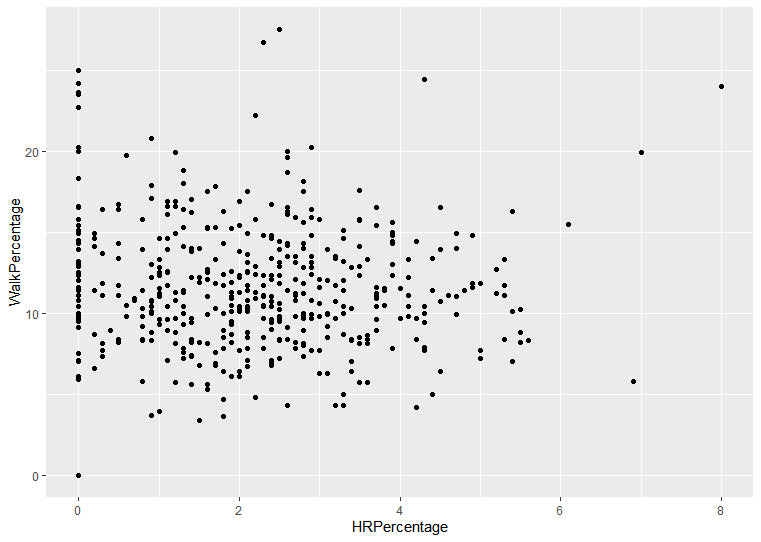
\includegraphics[width=0.5\linewidth]{PS6a_Matthies.png}
    \caption{}
    \label{fig:enter-label}
\end{figure}
%----------------------------------------------------------------------------

\vspace{1.5cm}


\includegraphics[scale=1.5]{}
\begin{figure}
    \centering
    \includegraphics[width=0.5\linewidth]{}
\begin{figure}
        \centering
        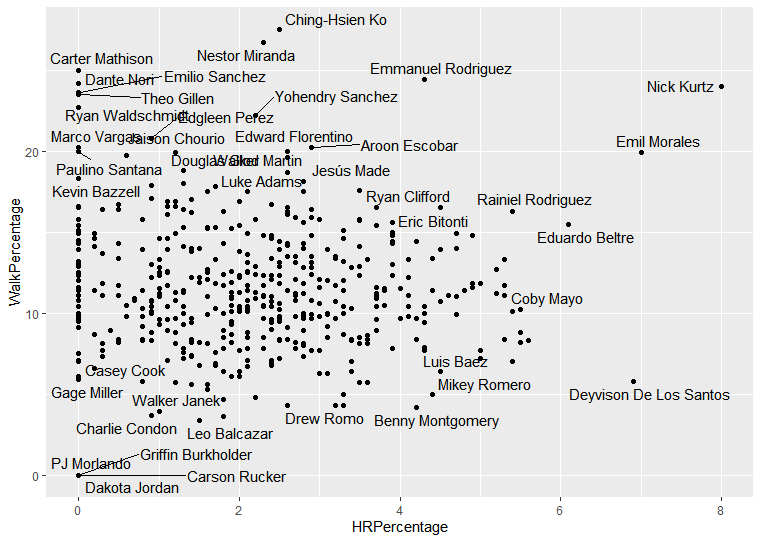
\includegraphics[width=0.5\linewidth]{PS6b_Matthies.png}
        \caption{}
        \label{fig:enter-label}
    \end{figure}
        \caption{}
    \label{fig:enter-label}
\end{figure}
%----------------------------------------------------------------------------

\newpage

%----------------------------------------------------------------------------


\includegraphics[width=5cm, height=4cm]{}
\begin{figure}
    \centering
    \includegraphics[width=0.5\linewidth]{}
\begin{figure}
        \centering
        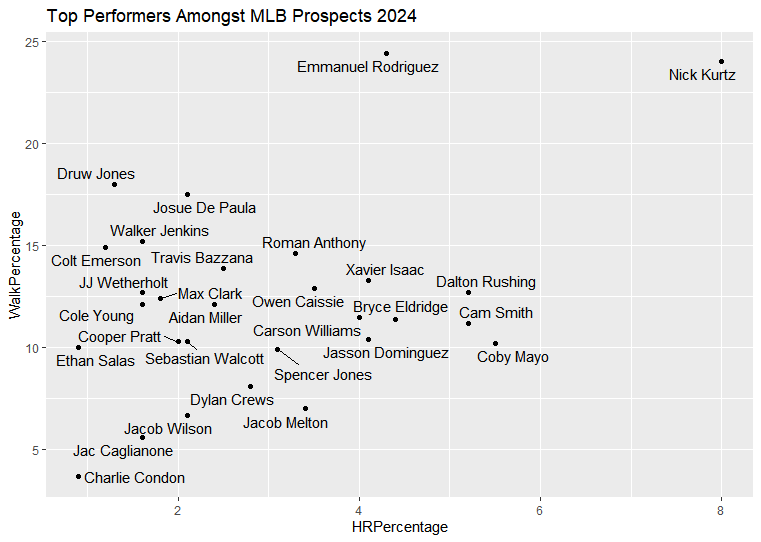
\includegraphics[width=0.5\linewidth]{PS6c_Matthies.png}
        \caption{Enter Caption}
        \label{fig:enter-label}
    \end{figure}
        \caption{}
    \label{fig:enter-label}
\end{figure}
%----------------------------------------------------------------------------

\vspace{1.5cm}

%----------------------------------------------------------------------------

\includegraphics[scale=1.2, angle=45]{}
\begin{figure}
    \centering
    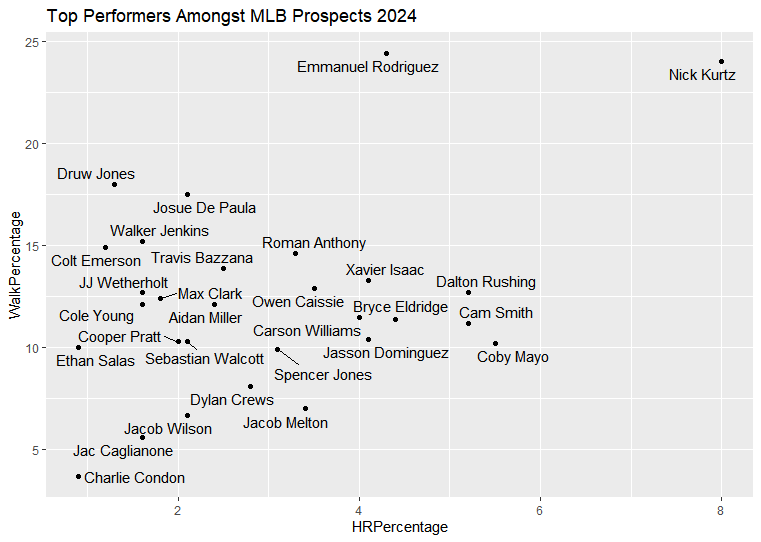
\includegraphics[width=0.5\linewidth]{PS6c_Matthies.png}
    \caption{Enter Caption}
    \label{fig:enter-label}
\end{figure}
%----------------------------------------------------------------------------


\end{document}


